\documentclass{article}

\usepackage[T1]{fontenc} % required for proper detokenization of \_

\usepackage{etoolbox}
\usepackage{tikz}
\usepackage{xifthen}

\usetikzlibrary
{
	matrix,
	fit,
}

\tikzset
{
	, RelationStyle/.style={draw}
	, AttributeNameStyle/.style={}
	, AttributeTypeStyle/.style={nodes={font=\small\scshape}}
	, PrimaryKey/.style={font=\bfseries}
	, Title/.style={font=\Large\itshape, inner ysep=1.5ex}
}

\newcommand\AttrList{}
\newcounter{AttributeCount}
\newcommand\clearAttrList
{
	\setcounter{AttributeCount}{1}
	\let\AttrList\empty
}

\newcommand\AddAttribute[3][]%
	% 1: Attribute Style
	% 2: Attribute Name
	% 3: Attribute Type
	{
		\stepcounter{AttributeCount}
		\xappto\AttrList{#1/#2/#3/\arabic{AttributeCount},}
	}

\newenvironment{Relation}[2][]
	{
		\clearAttrList{}
		\def\RelationTitle{#2}
		\tikzset{CustomRelationStyle/.style={#1}}
		
		% detokenize \_ so that underscores can be used in attribute names
		% (matching \endgroup in \end{env})
		\begingroup
		\catcode`_=11
	}
	{
		\let\matrixcontent\empty
		\foreach \attrStyle/\attrName/\typeName/\index in \AttrList
		{
			% Account for the trailing comma
			\ifthenelse{\equal{\index}{}}
			{
				% pass
			}
			{
				\xappto\matrixcontent
				{
					|[ \expandonce{\attrStyle} ]|
					\expandonce{\attrName \&}
					\expandonce{\typeName \\}
				}
			}
		}
		
		\matrix(\RelationTitle)
			[
				RelationStyle
				, CustomRelationStyle
				, nodes={minimum height=1em}
				, column 1/.style={anchor=base west, AttributeNameStyle}
				, column 2/.style={anchor=base west, AttributeTypeStyle}
				, matrix of nodes
				, nodes in empty cells
				, ampersand replacement=\&
			]
		{
			|[Title]| \RelationTitle \\
			\matrixcontent
		};
		
		% Draw a node for each attribute, encompasing both the name and type.
		\foreach \attrStyle/\attrName/\typeName/\index in \AttrList
		{
			% Account for the trailing comma
			\ifthenelse{\equal{\index}{}}
			{
				% pass
			}
			{
				\node (\RelationTitle-\attrName)
				[
					inner sep=0
					, fit =
						(\RelationTitle-\index-1.north west -| \RelationTitle.north west)
						(\RelationTitle-\index-2.south east -| \RelationTitle.north east)
				] {};
			}
		}

		% end group for detokenizing \_ (started at \begin{env})
		\endgroup
	}






% Tests %%%%%%%%%%%%%%%%%%%%%%%%%%%%%%%%%%%%

\usetikzlibrary
{
	positioning,
}

\begin{document}
	hello world

	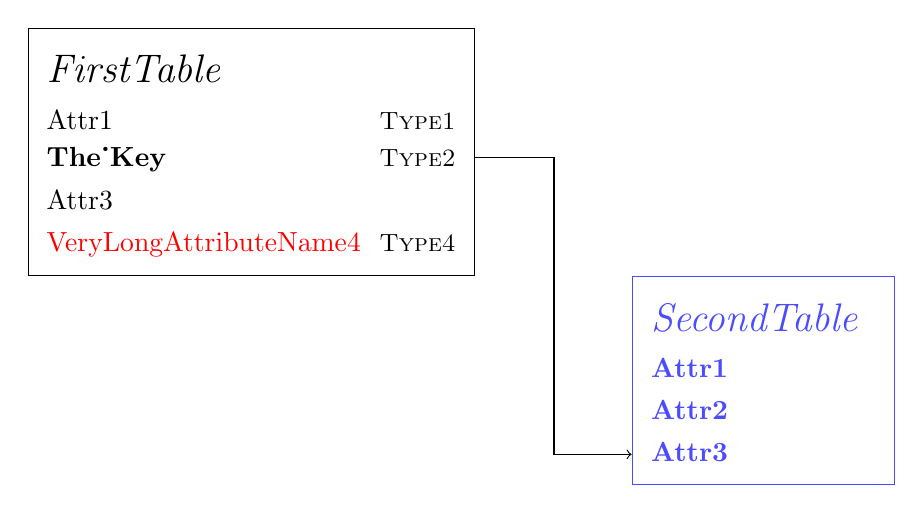
\begin{tikzpicture}[]
		\begin{Relation}{FirstTable}
			\AddAttribute{Attr1}{Type1}
			\AddAttribute[PrimaryKey]{The_Key}{Type2}
			\AddAttribute{Attr3}{}
			\AddAttribute[red]{VeryLongAttributeName4}{Type4}
		\end{Relation}

		\begin{Relation}
			[
				color=blue!70
				, below right=0 and 2 of FirstTable.south east
				, nodes={font=\bfseries}
			]{SecondTable}
			\AddAttribute[PrimaryKey]{Attr1}{}
			\AddAttribute[PrimaryKey]{Attr2}{}
			\AddAttribute{Attr3}{}
		\end{Relation}

		\draw[->] (FirstTable-The_Key.east) -- +(1,0) |- (SecondTable-Attr3.west);
		
	\end{tikzpicture}

	underscore\_still\_works\_in\_text\_and\_math
	\begin{equation}
		x_2 = \phi
	\end{equation}
		

	% Customize styles
	\tikzset
	{
		Title/.style={red,font=\ttfamily}
		, PrimaryKey/.style={font=\itshape\bfseries,blue}
		, Other/.style={green}
	}

	\begin{tikzpicture}
		\begin{Relation}[font=\ttfamily]{Custom Styles}
			\AddAttribute{foo}{bar}
			\AddAttribute[PrimaryKey]{foo_2}{bar}
			\AddAttribute[Other]{foo}{}
		\end{Relation}
		
	\end{tikzpicture}
	

	\end{document}
